So now we get to roughly deriving the Einstein field equations. A few notes: this is not at all rigorous. At points, you may wonder why we are doing
something, but it will come back to the equations. I will try to provide as much intuition as possible, but you will need to understand
at least a decent amount of what we have done so far. So, here goes.
\subsection{Metric Tensor}
Let's start by imagining a grassy field, something like the one shown below.
\begin{figure}[H]
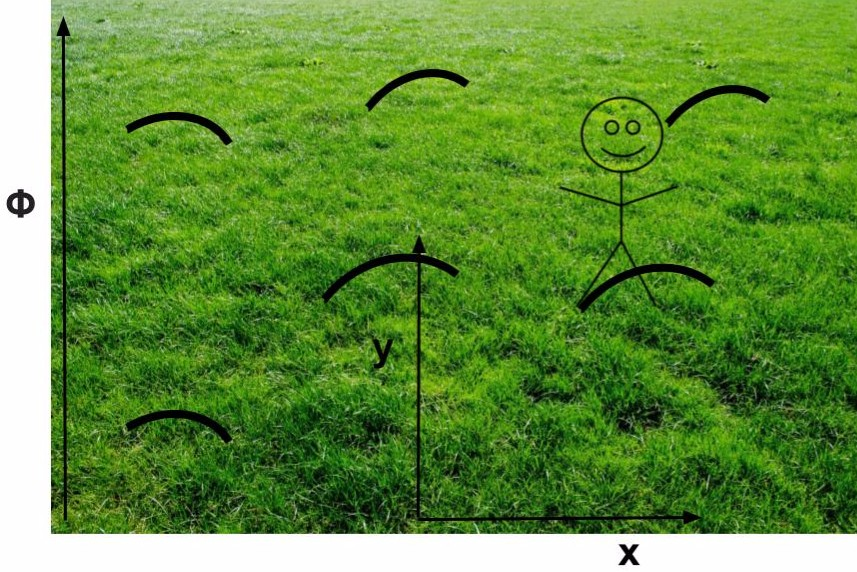
\includegraphics[scale=0.25]{field.jpg}
\end{figure}
